
%(BEGIN_QUESTION)
% Copyright 2011, Tony R. Kuphaldt, released under the Creative Commons Attribution License (v 1.0)
% This means you may do almost anything with this work of mine, so long as you give me proper credit

Suppose a FOUNDATION Fieldbus pressure transmitter will be used to measure pressure in a process vessel.  The transmitter will be connected to the vessel through a liquid-filled capillary tube connected to the ``High'' port.  The difference in height between the isolation diaphragm and the transmitter causes 1.7 PSI less pressure (i.e. 1.7 PSI of vacuum) to be applied to the transmitter's ``High'' port (due to the weight of the fill fluid) relative to the actual pressure inside the vessel.  In other words, with zero pressure inside the vessel, the transmitter will sense -1.7 PSI.

The transmitter needs to be ranged so that a pressure range of 50 to 100 PSI of gas pressure inside the vessel displays as 50 to 100 PSI to any operator looking at the DCS display, without the pressure error (offset) caused by the liquid-filled capillary tube.

$$\includegraphics[width=15.5cm]{i01839x01.eps}$$

Complete the configuration table in the above illustration, showing the proper {\tt XD\_Scale}, {\tt OUT\_Scale}, and {\tt L\_Type} parameter values to make the transmitter function as it should in this application.

\vfil 

\underbar{file i01839}
\eject
%(END_QUESTION)





%(BEGIN_ANSWER)

This is a graded question -- no answers or hints given!

%(END_ANSWER)





%(BEGIN_NOTES)

A good problem-solving technique for this scenario is to envision two ``thought experiments'': one where the vessel is at an actual pressure of 50 PSI, and another where the vessel is at an actual pressure of 100 PSI.  In each case, how much pressure does the transmitter see at its port?  In each case, what do we want the transmitter to output to the operator display?

\vskip 10pt

When the vessel is at 50 PSI, the transmitter will see 1.7 PSI less than that, or 48.3 PSI.  However, we want the operator to see ``50 PSI'' on the display, representing actual pressure inside the vessel.

\vskip 10pt

When the vessel is at 100 PSI, the transmitter will see 1.7 PSI less than that, or 98.3 PSI.  However, we want the operator to see ``100 PSI'' on the display, representing actual pressure inside the vessel.

\vskip 10pt

Thus, the transducer's sensed pressure range of 48.3 PSI to 98.3 PSI will become our {\tt XD\_Scale} while the desired (displayed) pressure range of 50 PSI to 100 PSI will become our {\tt OUT\_Scale}.  The AI function block performing this scaling will automatically calculate the $y = mx + b$ equation parameters necessary to scale from one range to the other, so long as we leave its linearization type set to {\tt Indirect}:

\vskip 10pt

{\tt XD\_Scale} = 48.3 to 98.3 PSI

\vskip 10pt

{\tt OUT\_Scale} = 50 to 100 PSI

\vskip 10pt

{\tt L\_Type} = Indirect

\vskip 10pt

Basically, the AI function block will implement a $y = mx + b$ equation of $\hbox{OUT} = \hbox{XD} + 1.7$ with these parameters.
%INDEX% Fieldbus, instrument ranging: setting XD_Scale and OUT_Scale parameters for an application

%(END_NOTES)

